\documentclass[a4paper,10pt,oneside]{scrreprt}
\usepackage[latin1]{inputenc}
\usepackage[english]{babel}
\usepackage{graphicx}
\usepackage{float}
\usepackage{geometry}
\geometry{verbose,a4paper,tmargin=15mm,bmargin=25mm,lmargin=15mm,rmargin=15mm}
\usepackage{paralist}

\usepackage{paracol}

\usepackage{todonotes}

\usepackage{listings}
\lstset{language=Java,
	tabsize=2,
	showspaces=false,
	showtabs=false,
	breaklines=true,
	showstringspaces=false,
	breakatwhitespace=true,
	commentstyle=\color{pgreen},
	keywordstyle=\color{pblue},
	stringstyle=\color{pred},
	basicstyle=\footnotesize\ttfamily,
	moredelim=[il][\textcolor{pgrey}]{$$},
	moredelim=[is][\textcolor{pgrey}]{\%\%}{\%\%}
}

\usepackage{tikz}
\usetikzlibrary{calc,patterns,angles,quotes}

\usepackage{caption}
\usepackage{subcaption}
\usepackage{tabularx} % in the preamble

\usepackage{pdfpages}

%\usepackage{indentfirst} % for always indenting the first paragraphs

\usepackage{wrapfig}
\usepackage{lipsum}
\usepackage[linewidth=1.2pt,linecolor=red]{mdframed} % for boxes around wrapfigure and text

\begin{document}


\begin{center}
	Submitted by Group 18

	\bigskip

	\begin{tabular}{c}
	Group Members: \\
	CETIN, Ulfet (391819); GRUCZKA, FILIP (413279);	LIPINSKI, Bartosz (413177) \\
	SZYMANSKI, Bartosz (411949); GONG, Zeheng (378125)\\
	\end{tabular}

	\bigskip

	DIS1 WS 19/20 - Project Milestone III\\
	Ideation - Phase II\\

	%	(ordered on lastname basis)
\end{center}
\vspace{-1cm}

\clearpage

\begingroup
\let\clearpage\relax
	\chapter{Storyboard walkthrough}
\endgroup


\section{Solution \#1:}

\begin{figure}[H]
	\centering
	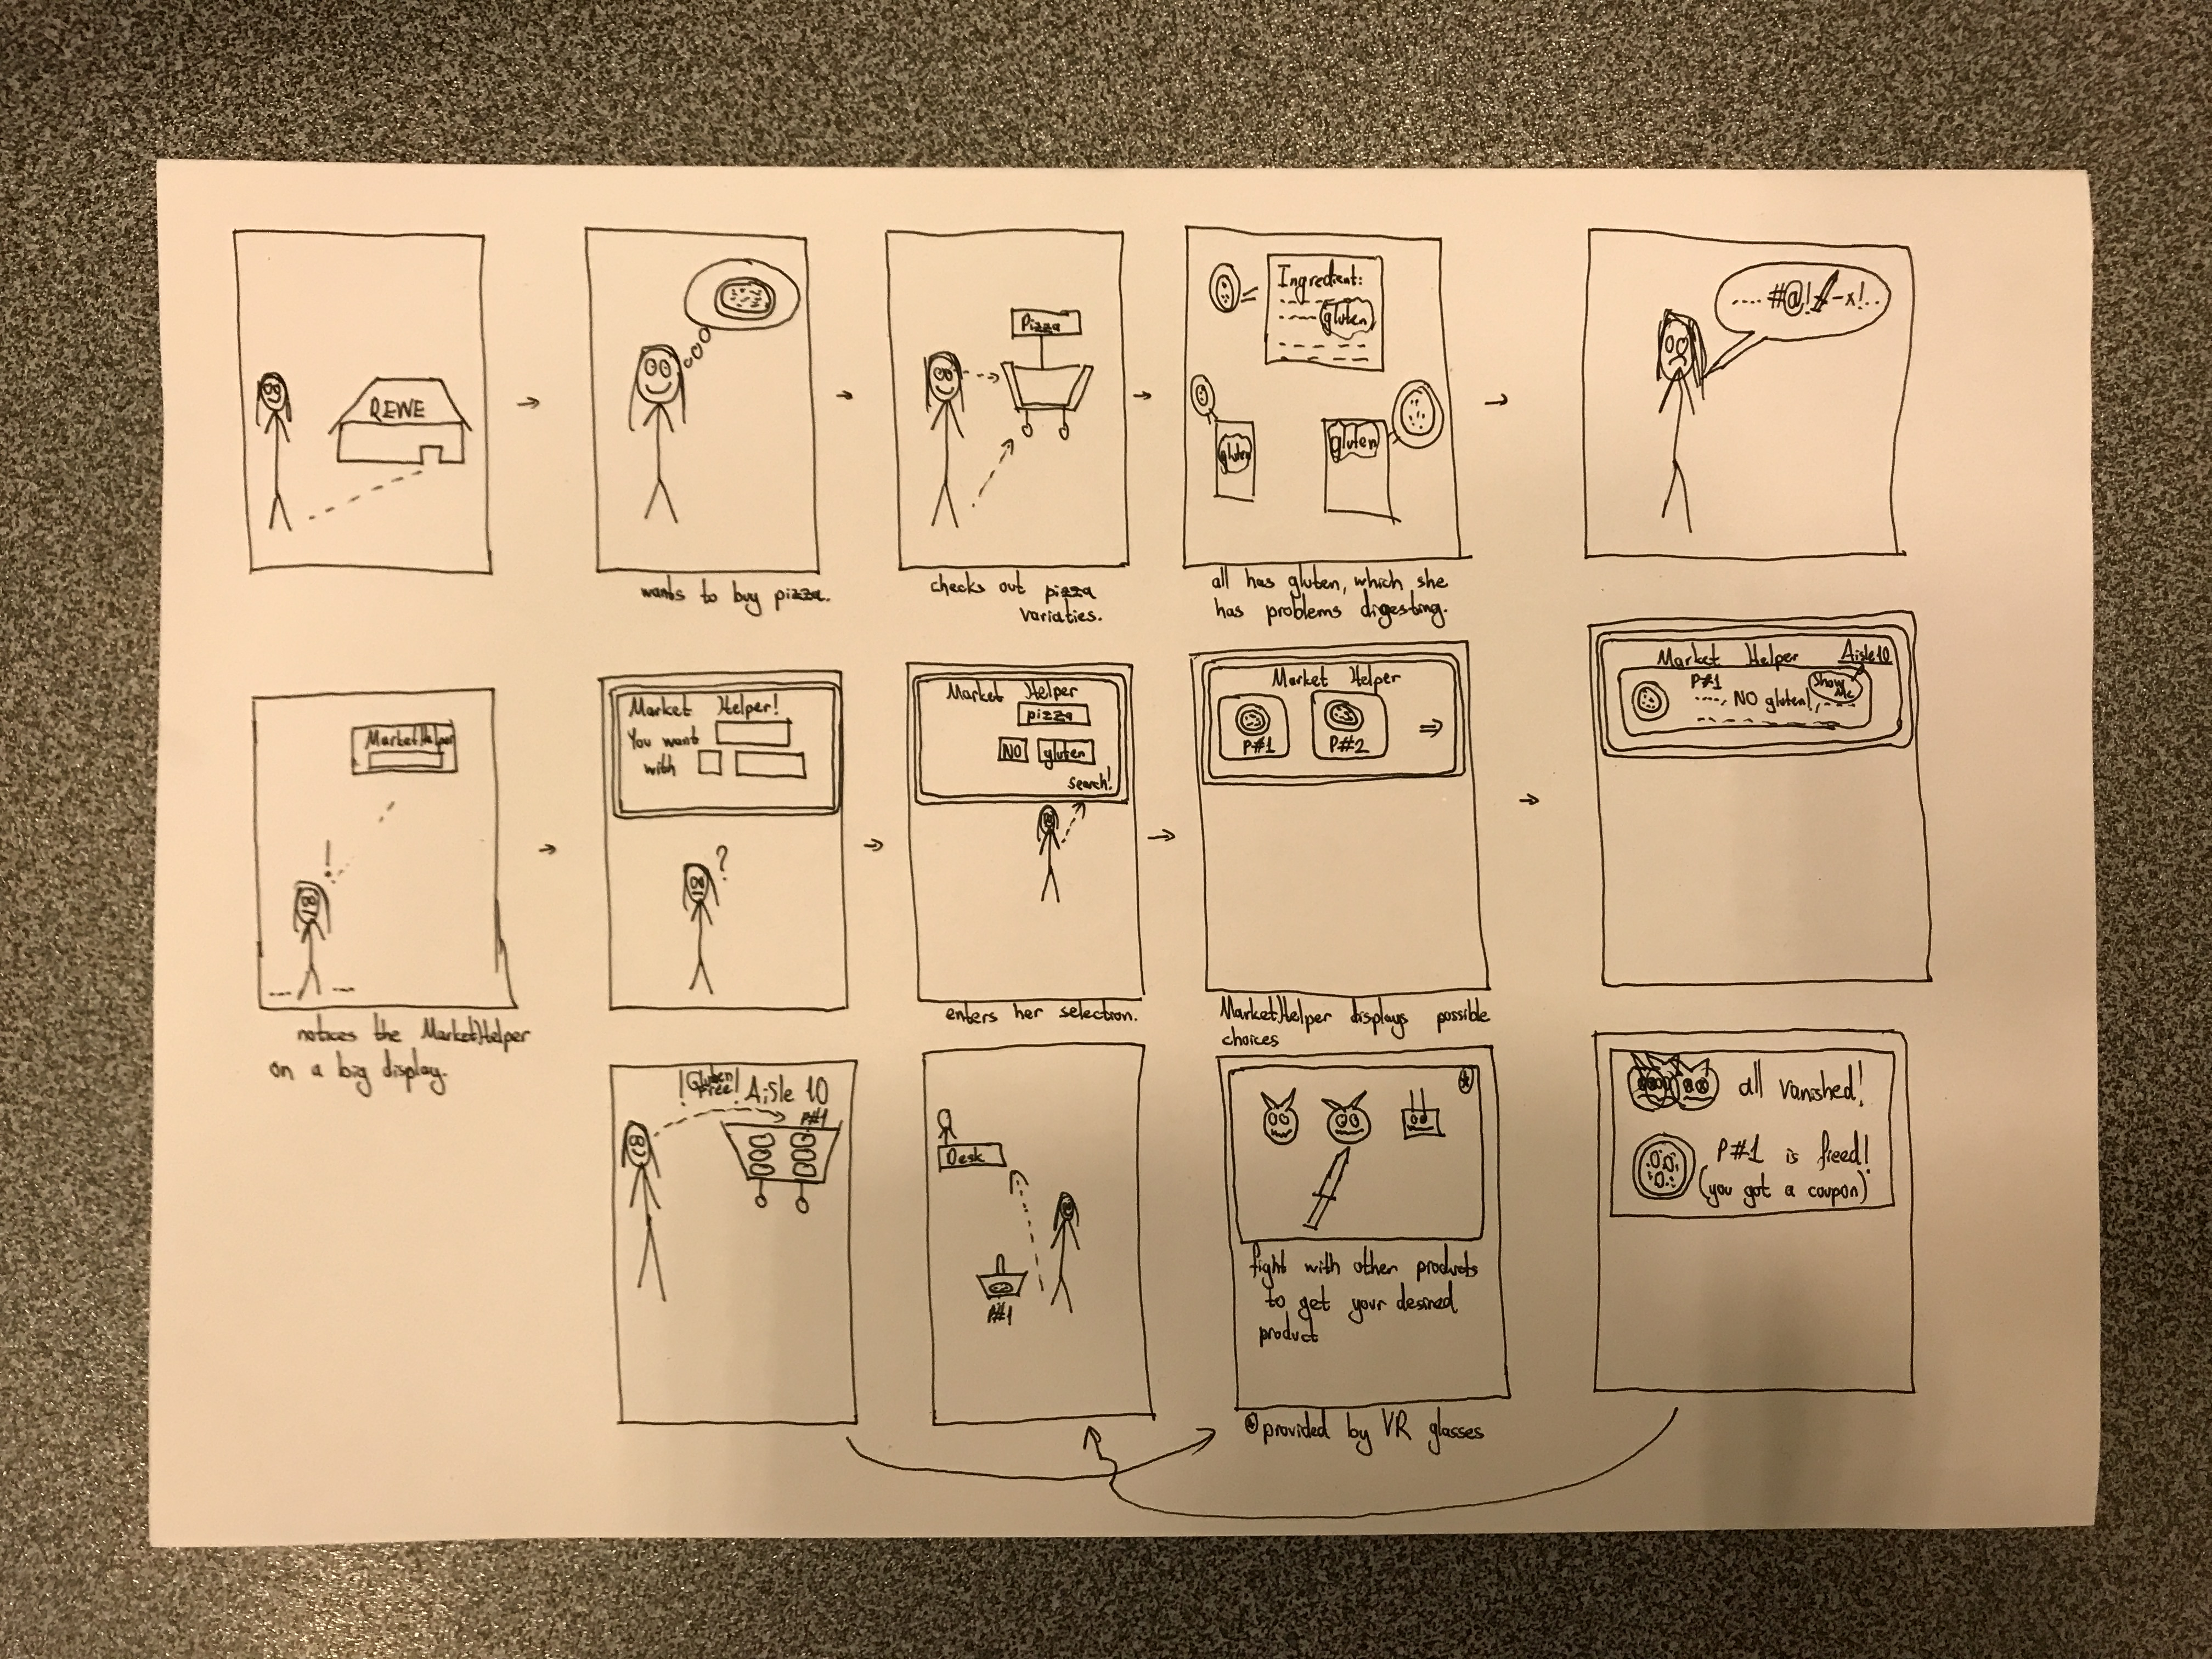
\includegraphics[scale=0.16, clip, trim={40em 28em 40em 33em}]{images/s1.jpg}
\end{figure}

User \#1:
\begin{compactitem}
	\item Name: Hakan
	\item Information: age of 23, Turkish
	\item Profession: M.Sc. student
	\item likes to  play games and hang out with friends
	\item representative of our third persona (David)
\end{compactitem}
\bigskip

Answers:
\begin{compactitem}
	\item Do the users understand the solution?\\
		Yes, it was clear for the user. The user also really likes the solution.\\
	
	\item Do the users find the solution realistic?\\
		Not so much. The other parts are really possible, while VR goggles part was not realistic at all: the fighting with the other mascots is silly, not everyone wants that (might be hard for elderly). But fighting for right-earned food might also be fun for some.\\
		
	\item Do the users feel that this solution can solve his/her problem(s)? If not, what is still
	a problem? Is there a solution that could solve this?\\
		Yes, especially when he wants to find some obscure ingredient that he needs to complete a recipe. It is also better than asking some retail worker. He agreed that it might solve his problem.
\end{compactitem}
\bigskip

Transcript of the User Study (shortened):\\

\noindent Q: (the solution is explained) Can you take a look first? On the first box you can see a girl, this girl has a specific condition, ..., she has to find a specific product (pizza with no gluten), yet it does not have to be about just some health condition.  \\
A: It is pretty clear from the drawings and also after you explained. I think it is a quite nice solution.\\
Q: Do you find the solution realistic?\\
A: To be honest, the part about VR goggles are not really realistic, but the parts before are quite realistic and possible. \\
Q: Why do you think so?\\
A: The fighting with the other mascots are for me silly, people do not want to fight each time they go shopping. Also, not good for elderly, for example, and it seems kinda silly.\\
Q: Do you think that people would find this fun? Did you find this idea fun?\\
A: It could be fun, yeah. You can just get into the game (like role-playing) and in the end, you get your hard earned food, but I do not think it is a viable solution here.\\
Q: Do you have such a problem (of finding the right food)\\
A: (explains his experience, especially about specific recipes calling for specific ingredients) This kind of thing would help. So yes.


\bigskip
\bigskip

User \#2:
\begin{compactitem}
	\item Name: Furkan
	\item Information: age of 26, Turkish
	\item Profession: M.Sc. student
	\item interested in fitness, likes to learn about anything, joining online courses, gym-going, reading a lot
	\item representative of our first persona (Picky Eater Helga Ratt)
\end{compactitem}
\bigskip

Answers:
\begin{compactitem}
	\item Do the users understand the solution?\\
		Yes, only the game part is not very clear. How is he going to kill the other mascots was not clear. One other question was whether VR goggles are going to provided by the market.\\
	
	\item Do the users find the solution realistic?\\
	He is both concerned about the number of available screens in the market and who would provide the VR goggles. In short, he does not find it that much realistic.\\
	
	\item Do the users feel that this solution can solve his/her problem(s)? If not, what is still
	a problem? Is there a solution that could solve this?\\
		He thinks this would not solve his problems in its current form. He would like to have it in a way that more than one item is searchable via the application, so we would not spend so much time in front of the screen. However, he finds this promising.\\
		(he is also curious whether people would be concerned about gazes of others, as this application would be out in the open and everyone would see what he searched for)\\
		He said playing games in home and coming to fetch the coupons would be more fun!
\end{compactitem}

\clearpage

\section{Solution \#2:}
\begin{figure}[h]
	\centering
	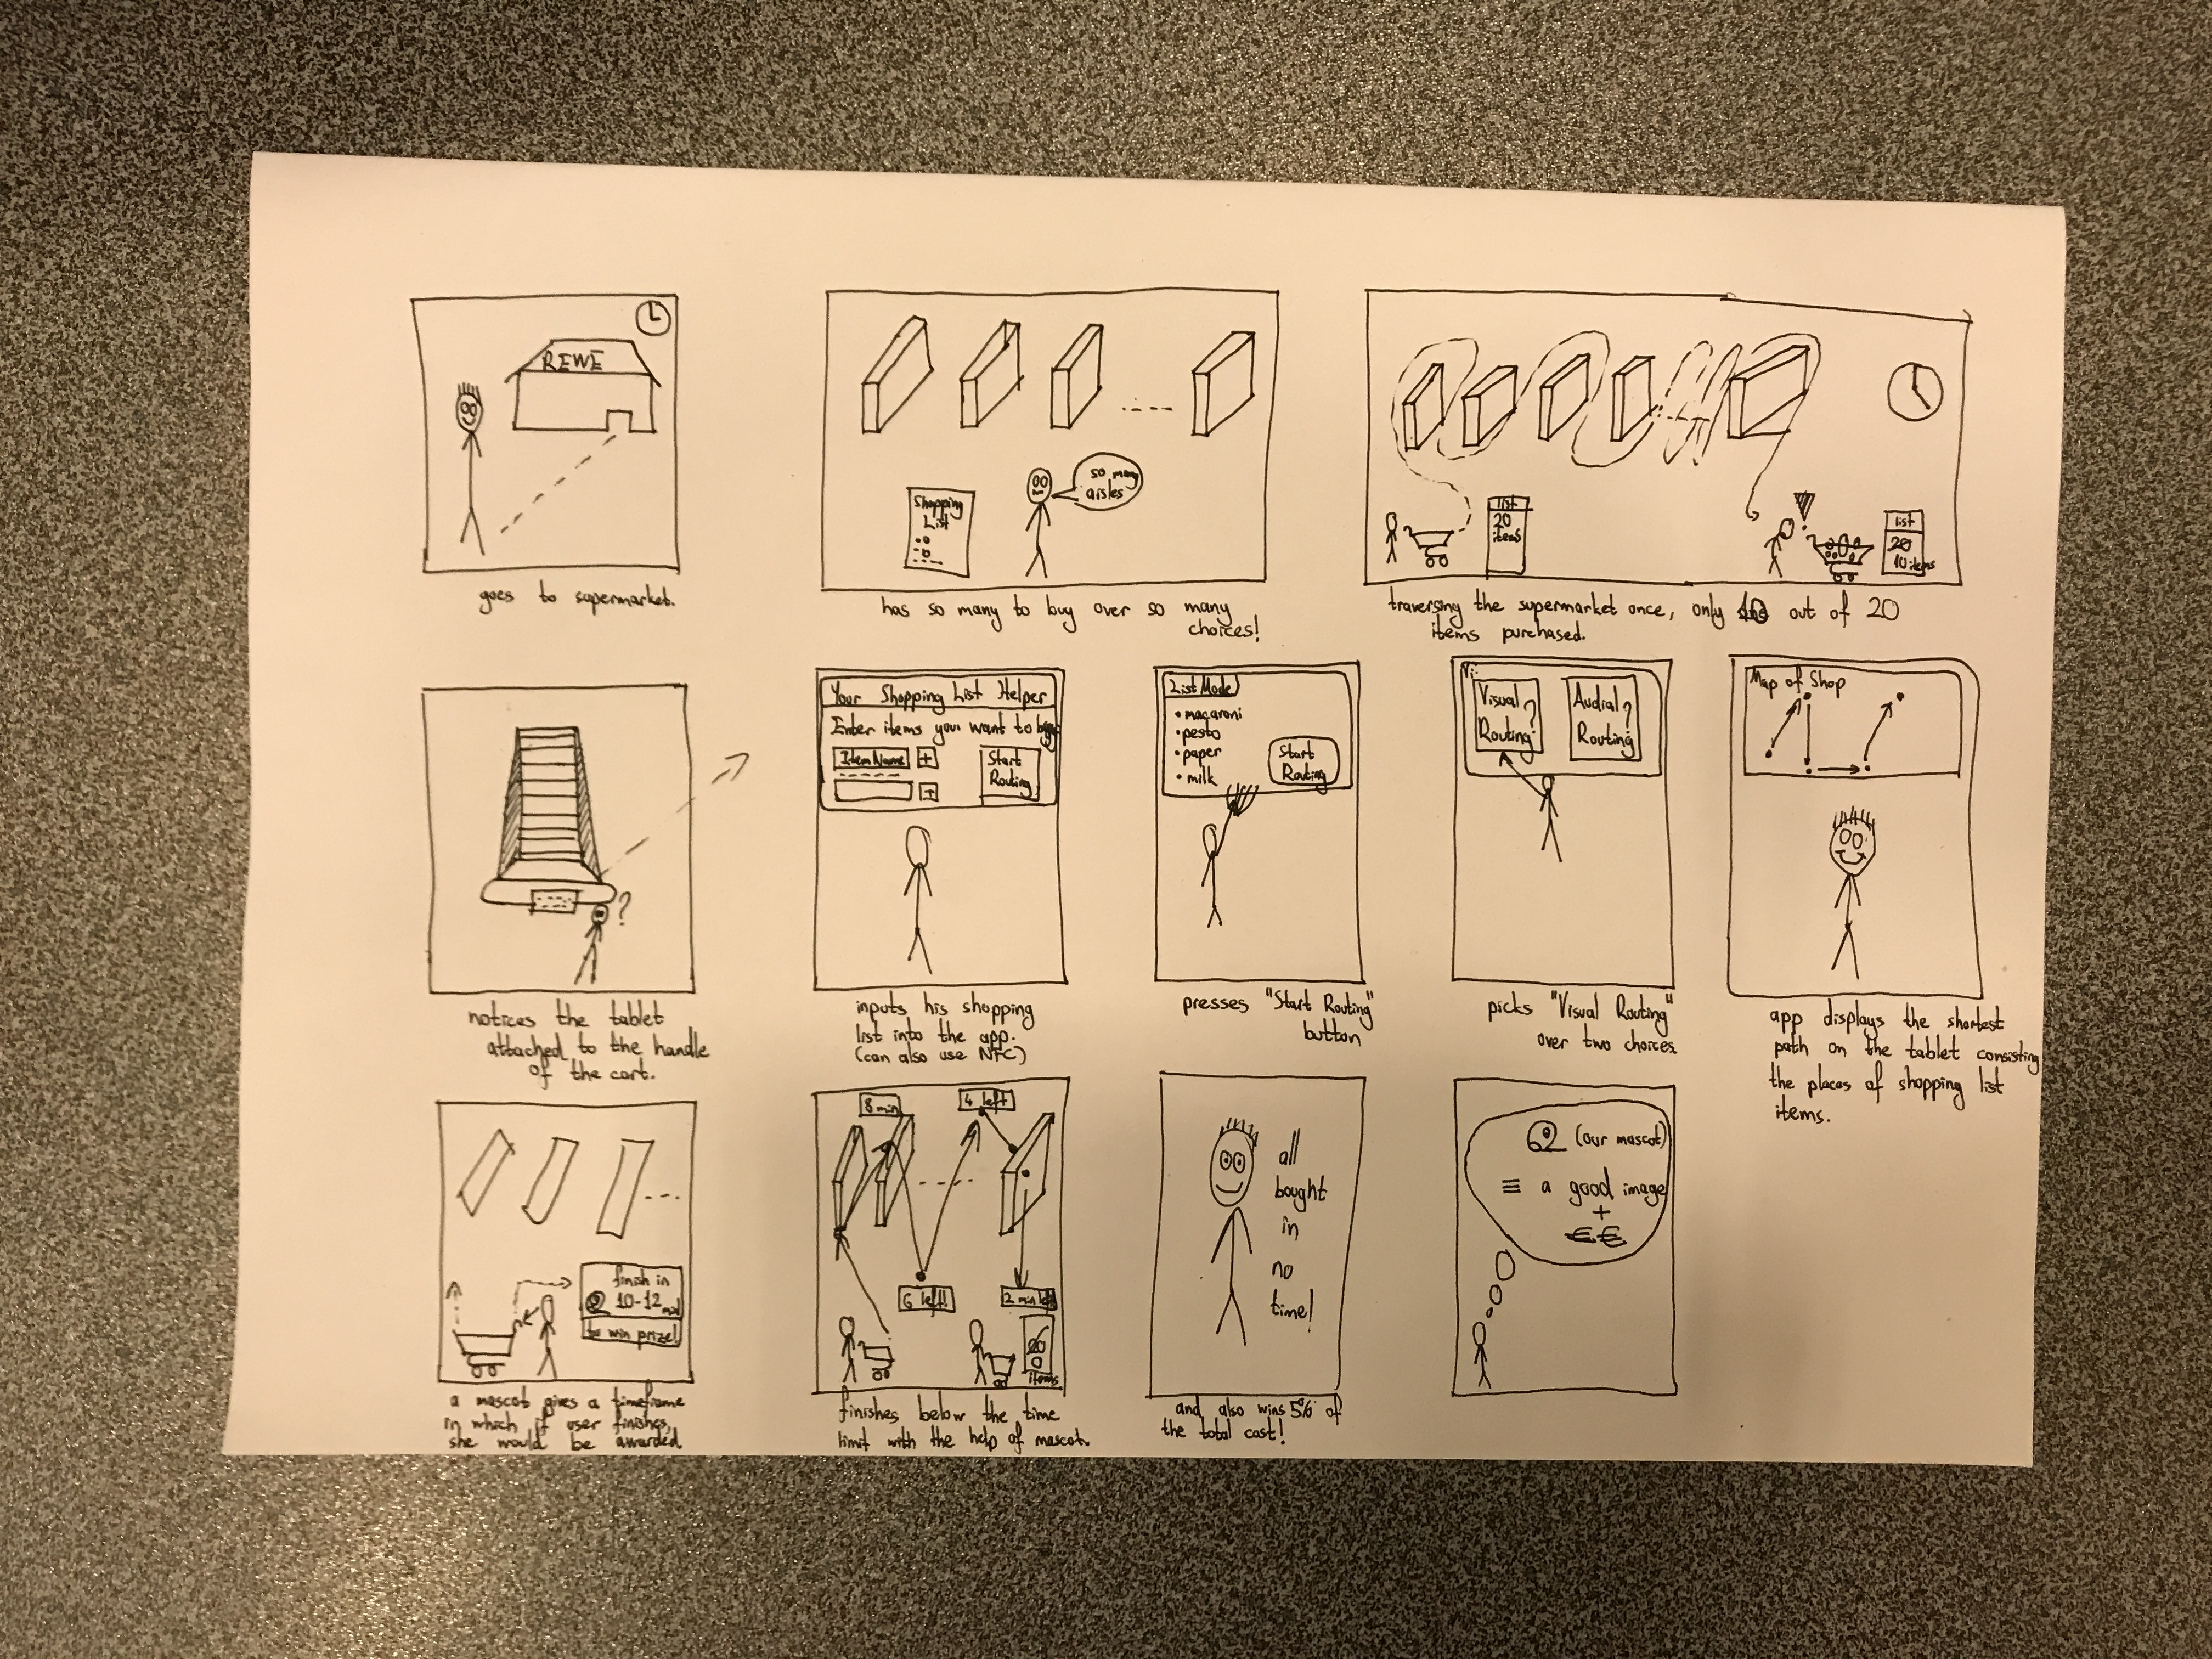
\includegraphics[scale=0.16, clip, trim={71em 35em 33em 43em}]{images/s2.jpg}
\end{figure}

User \#1:
\begin{compactitem}
	\item Name: Hakan
	\item Information: age of 23, Turkish
	\item Profession: M.Sc. student
	\item likes to  play games and hang out with friends
	\item representative of our third persona (David)
\end{compactitem}
\bigskip

Answers:
\begin{compactitem}
	\item Do the users understand the solution?\\
	Yes, it is quite clear. The user were able to explain the solution completely by putting himself in the shoes of the example in the storyboard.\\
	
	\item Do the users find the solution realistic?\\
	Much more realistic than the Solution \#1. Also, he finds this solution innovative to come up with.\\
	
	\item Do the users feel that this solution can solve his/her problem(s)? If not, what is still
	a problem? Is there a solution that could solve this?\\
	Yes, definitely. He also goes around the shop and got bored afterwards seeing all the same places, and this would really improve his experience.\\
\end{compactitem}
\bigskip

\noindent Q: (solution explained) The storyboard is a bit obscure (the candidate agrees). You can choose a routing based on your preference. (...) In a time range, if the customer goes to the cash desk, with the mascot cherishing for you. Do you understand the solution?\\
A: Yes, quite clearly. (the user explains in a short manner)\\
Q: Do you find the solution realistic?\\
A: Yes, especially compared to the solution \#1. As long as the layout of the shop significantly changes, it is pretty innovative thing to come up with.\\
Q: Do you find the solution fun?\\
A: Yes, unlike the first one, it does not interfere with my shopping, and if I am fast enough, and with a coupon that is a positive feedback, that is actually pretty good.\\
Q: (some extra questions on usability)


\bigskip
\bigskip

User \#2:
\begin{compactitem}
	\item Name: Furkan
	\item Information: age of 26, Turkish
	\item Profession: M.Sc. student
	\item interested in fitness, likes to learn about anything, joining online courses, gym-going, reading a lot
	\item representative of our first persona (Picky Eater Helga Ratt)
\end{compactitem}
\bigskip

Answers:
\begin{compactitem}
	\item Do the users understand the solution?\\
	Yes, user understands the solution and can explain the solution with his own words.
	\\
	
	
	\item Do the users find the solution realistic?\\
	Yes, but the user finds it not so viable for the supermarket, as supermarkets want the customers to spend more time inside, so the customers would buy more.
	\\
	
	\item Do the users feel that this solution can solve his/her problem(s)? If not, what is still
	a problem? Is there a solution that could solve this?\\
	Yes, the user agrees that this product would solve his problem, yet he is curious about the approaches of the supermarkets towards this product. Moreover, he does not want to be seen running around for coupons (it is explained that there would be time frame, so no early finishers would be gifted coupons)
	\\
\end{compactitem}
\bigskip

\noindent Q: (solution explained as before) \\
A: (finds the mascot not decipherable, explains the solution in his words) \\
Q: Do you find the solution realistic?\\
A: Realistic, but one catch: there is a product like that. It is also counterproductive in the sense of supermarket, they want people to spend money. Good for the customer, not so good for the supermarket.\\
Q: Do you think that this solution can solve your problem?\\
A: Definitely. Would help me in my shopping, no doubt.\\
Q: Would it be more fun? \\
A: Nobody would like to look cheap running around (we explained that there would be a timeframe, not would be a race to go earlier)\\



\clearpage
\section{Solution \#3:}

\clearpage
\section{Solution \#4:}

\clearpage
\section{Solution \#5:}

\clearpage
\section{Solution \#6:}

\chapter{Our Evaluation}

Selected Solutions:\\

\section{Solution \#x:}

\section{Solution \#y:}

\section{Solution \#z:}

\chapter{Final Storyboards}
				
\end{document}}
